\documentclass[xcolor=dvipsnames]{beamer}

\usepackage{setspace}
\usepackage{amsmath}
\usepackage{float}
\usepackage{longtable}
\usepackage{booktabs}
\usepackage{lscape}
\usepackage{graphicx}
\usepackage{silence}
\usepackage{forest}
\usepackage{hyperref}
\usepackage{placeins}
\usepackage{xcolor}
\usepackage{textcomp} % Needed on Windows in Office
\usepackage{derivative}
\usepackage{adjustbox}
\usepackage{tabularx}

\usepackage[style=apa]{biblatex}

\makeatletter
\g@addto@macro\normalsize{%
	\setlength\abovedisplayskip{0pt}
	\setlength\belowdisplayskip{-0pt}
}


\linespread{1.5}\selectfont

\usepackage[toc,page]{appendix}


\let\Oldsubsection\subsection
\renewcommand{\subsection}{\FloatBarrier\Oldsubsection}

\graphicspath{{05.Figures/}}

\bibliography{airline}

\author{Ann Atwater}
\institute{University of Florida}

\title{Distributional Effects of Mergers}
\subtitle{Evidence from the Attempted JetBlue-Spirit Merger}
\date{September 2, 2025}

\usetheme{Berkeley}

\begin{document}
	\section{Introduction}
	\frame{\titlepage}
    \begin{frame}
        \frametitle{Motivation}
        \begin{itemize}
            \item Horizontal mergers simultaneously possess pro-consumer and anti-consumer aspects.
            \begin{enumerate}
                \item Pro-Consumer: Shifting of assets from less productive uses to more productive uses, realization of economies of scale create more effective, competitive firms (\cite{williamson_economies_1968, farrell_horizontal_1990, kaplow_improving_2025})
                \item Anti-Consumer: Two former rivals operate in a state of perfect collusion, creating lower competition. (\cite{stigler_theory_1964})
            \end{enumerate}
        \end{itemize}
    \end{frame}

    \begin{frame}
        \frametitle{Motivation}
        \begin{itemize}
        \item As such, horizontal mergers may be good or bad for the overall economy.
            \item Globally, antitrust regulators focus on consumer welfare to guide merger approval decisions. 
            \begin{itemize}
                \item Do the pro-consumer aspects outweigh the anti-consumer forces within a given merger. 
        \end{itemize}
        \item In general - mergers of larger firms are presumed anti-competitive.
        \end{itemize}
    \end{frame}

    \begin{frame}
        \frametitle{Motivation}
        \begin{itemize}
            \item Throughout the economy, firms are heterogeneous in their customer bases.
            \begin{enumerate}
                \item Consumer Preferences: Vegan, Fast-Food, Steakhouses 
                \item Consumer Willingness to Pay: Legacy, Low-Cost Carrier, Ultra-Low-Cost Airlines
            \end{enumerate}
            \item Latter of these is the focus of this paper. 
        \end{itemize}
    \end{frame}

    \begin{frame}
    \frametitle{Questions}
        \begin{itemize}
        \item How does a merger of two firms which target different consumer segments impact overall consumer welfare?
        \item How do mergers effect different groups of consumers?
        \item Was the proposed JetBlue-Spirit merger pro-consumer?
        \item How did the covid-19 pandemic change the airline industry?
        \end{itemize}   
    \end{frame}

    \begin{frame}
        \frametitle{Preview of Results}
        \begin{itemize}
            \item 
        \end{itemize}
    \end{frame}

    \begin{frame}
		\frametitle{Literature Review}			\begin{itemize}
				\item Anti-competitive Conduct in Aviation (\cite{miller_did_2010, zou_assessing_2023})
				\item Aviation Mergers 
				\begin{itemize}
					\item Completed Mergers (\cite{luo_price_2014, carlton_are_2019})
					\item Simulated Mergers (\cite{ciliberto_market_2021, li_repositioning_2022})
				\end{itemize}
				\item Understanding Aviation Industry
				\begin{itemize}
					\item Role of Low-Cost Carriers (\cite{goolsbee_how_2008, shrago_spirit_2024})
					\item Post-Pandemic Changes (\cite{zou_assessing_2023, ewen_zoom_2023})
				\end{itemize}
        \end{itemize}
	\end{frame}
	
	\begin{frame}
		\frametitle{Presentation Roadmap}
		\begin{enumerate}
				\item Setting
				\begin{itemize}
					\item American Aviation Industry
					\item JetBlue-Spirit Merger
				\end{itemize}
				\item Data and Summary Statistics
				\item Model and Results 
				\begin{itemize}
					\item Demand Model
                    \item Supply Model
                    \item Merger Simulations
                    \item Consumer Surplus
				\end{itemize}
                \item Conclusion
			\end{enumerate}
	\end{frame}

    \section{Setting}
	\begin{frame}
		\frametitle{Types of Carrier}
		\begin{itemize}
			\item Three Types:
			\begin{itemize}
				\item Legacy % (Existed Pre-1978 Deregulation)
				\item Low-Cost 
				\begin{itemize}
					\item Exemplified by Southwest Airlines
					\item Focus on Direct Flights
				\end{itemize}
				\item Ultra-Low Cost
				\begin{itemize}
					\item Introduced by Spirit in 2010
					\item `Unbundled' Tickets
				\end{itemize}
			\end{itemize}
		\end{itemize}
	\end{frame}
	
	\begin{frame}
		\frametitle{Legacy Carriers}
		\begin{itemize}
			\item At present, Delta, United, and American
			\item Characterized by higher fares, costs than the other carrier types
			\item ``Hub-And-Spoke" Route Networks connect passengers from smaller markets to centralized hubs before another flight to the final destination.
			\begin{itemize}
				\item Firms have large costs of running these hubs and operate a wider variety of aircraft within their fleets
			\end{itemize}
		\end{itemize}
	\end{frame}
	
	\begin{frame}
		\frametitle{Low-Cost Carriers}
		\begin{itemize}
			\item Major low-cost carriers include Southwest and JetBlue
			\begin{itemize}
				\item Southwest is the largest low-cost carrier and originator of the model within the United States
			\end{itemize}
			\item Focus on  direct flights between larger markets to reduce costs, fares
			\item This allows for streamlined fleets to reduce training, maintenance expenses
		\end{itemize}
	\end{frame}
	
	\begin{frame}
		\frametitle{Ultra-Low Cost Carriers}
		\begin{itemize}
			\item Spirit, Allegiant, and Frontier
			\item ``Unbundled Fares" - Traditional Amenities are now an extra fare on top of the seat price.
			\begin{itemize}
				\item Spirit was the first ULCC in the United States
				\item Dates to April 2010 decision to charge for checked baggage. 
			\end{itemize}
		\end{itemize}
	\end{frame}    

    \begin{frame}
        \frametitle{Airline Industry After Covid-19}
        \begin{itemize}
            \item The Covid-19 Pandemic Caused a Large Decrease in Air Travel
            \item Industry saw recovery to roughly 2016 levels of air travel in 2021Q2, after widespread vaccine availability.
            \item Changes in Ridership Go Beyond Levels
        \end{itemize}
    \end{frame}

    \begin{frame}
        \frametitle{Quarterly Ridership, All Carriers}
        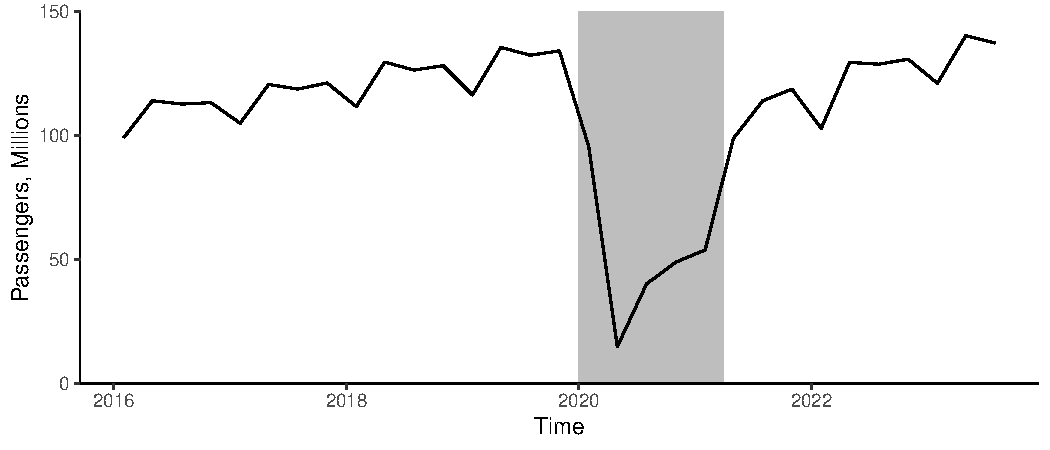
\includegraphics[width = \linewidth]{Quarterly_DB1B_Itineraries}
    \end{frame}


    \begin{frame}
        \frametitle{Airline Industry After Covid-19}
        \begin{itemize}
         \item Consumer Base of Industry Changed
            \begin{itemize}
                \item Business Travelers Historically Roughly Third of Riders
                \begin{itemize}
                    \item Less Price Sensitive than Leisure Travelers
                \end{itemize}
                \item Business Travel Did Not Immediately Recover Post Pandemic
                \item Simultaneously: Leisure Travelers Built Up Cash Returns
                \begin{itemize}
                    \item Revenge Travel
                \end{itemize}
                \item Demand Elasticity Change Apriori Ambiguous
            \end{itemize}
        \end{itemize}
    \end{frame}


    \begin{frame}
        \frametitle{JetBlue}
        \begin{itemize}
            \item Second largest Low-Cost Carrier in the United States, behind Southwest
            \item Primarily in Markets on the Eastern Seaboard
            \item Increasingly Anti-Competitive Conduct
            \begin{itemize}
                \item Northeast Alliance with American Airlines - Coordination in Four Airports (NYC, Boston areas)
            \end{itemize}
            \item Saw Purchasing Spirit As Way to Bolster Fleet
            \begin{itemize}
                \item Both Fleets Primarily Airbus A320, but in Different Seating Configurations
            \end{itemize}
        \end{itemize}
    \end{frame}

    \begin{frame}
        \frametitle{JetBlue, Spirit Fleet Sizes}
        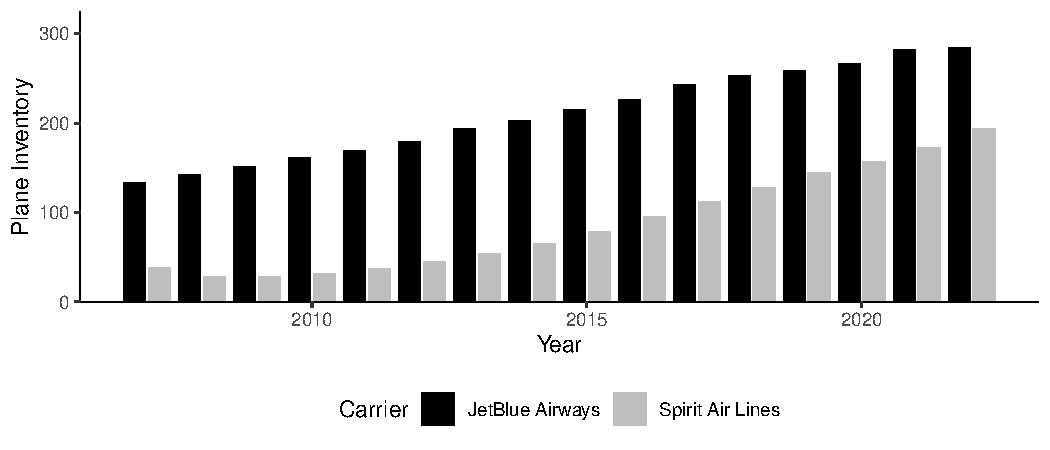
\includegraphics[width = \linewidth]{Both_Planes.pdf}
    \end{frame}


    \begin{frame}
        \frametitle{Spirit}
        \begin{itemize}
            \item Largest Ultra-Low Cost Carrier in the United States
            \item Focused on budget conscious travelers
            \item Dramatic growth during the 2010s, through the pandemic
            \item Non-Fare ``ancillary fees" for its ``unbundled" tickets
            \begin{itemize}
                \item Checked Baggage Fees, Online Booking Fees, etc.
            \end{itemize}
        \end{itemize}
    \end{frame}

    \begin{frame}
     \frametitle{Spirit - Revenue Sources over Time}
        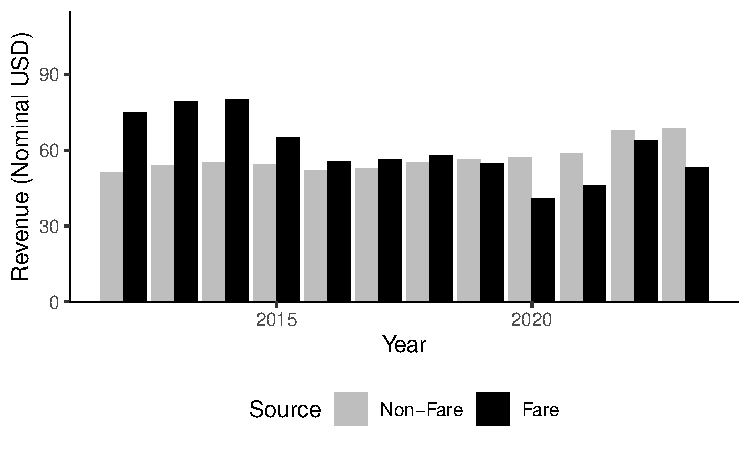
\includegraphics[width = \linewidth]{05.Figures/Spirit_Revenue_Sources.pdf}
    \end{frame}

    \begin{frame}
        \frametitle{JetBlue-Spirit Merger}
    \end{frame}


    \section{Data and Summary Statistics}

    \begin{frame}
		\frametitle{Data}
		\begin{itemize}
			\item Airline Origin and Destination Survey (DB1B)
			\begin{itemize}
				\item 10\% Sample of Domestic Passenger Itineraries 
				\item Data on Origin, Destination, Fare, Route, Carrier
                \item Ancillary Fees Not Included 
			\end{itemize}
		\end{itemize}
	\end{frame}

    % Consequence of No-Ancillary Fees as Slide?

    \begin{frame}
        \frametitle{Market, Product Definitions}
        \begin{itemize}
        	\item Markets defined as Year-Quarter-Origin-Destination 
			\item Market Size is the Geometric Mean of the Population of Origin, Destination Metropolitan Statistical Areas
			\item Products Further Defined by Carrier, Nonstop Status
        \end{itemize}
    \end{frame}

      \begin{frame}
        \frametitle{Summary Statistics - Product Level}
                \begin{adjustbox}{max height=\dimexpr\textheight-5.5cm\relax,
           max width=\textwidth}

\begin{tabular}[t]{llllll}
\toprule
 & Mean & (SD) & Minimum & Median & Maximum\\
\midrule
\addlinespace[0.3em]
\multicolumn{6}{l}{\textbf{Pre-Pandemic}}\\
\hspace{1em}Price (2017 USD) & 233.37 & (68.47) & 33.12 & 235.76 & 810.58\\
\hspace{1em}Price (Nominal USD) & 237.78 & (69.7) & 34 & 240.27 & 821.77\\
\hspace{1em}Passengers & 4248.33 & (10185.27) & 100 & 810 & 192050\\
\hspace{1em}Distance (1000s) & 1.41 & (0.67) & 0.15 & 1.28 & 3.87\\
\hspace{1em}Extra Distance & 0.13 & (0.18) & 0 & 0.06 & 1.66\\
\hspace{1em}Nonstop & 0.28 & (0.45) & 0 & 0 & 1\\
\hspace{1em}Origin Destinations & 29.97 & (33.37) & 1 & 13 & 180\\
\hspace{1em}Origin Presence (\%) & 36.23 & (31.26) & 0.54 & 19.51 & 100\\
\midrule
\hspace{1em}Observations & 307849 &  &  &  & \\
\bottomrule
\end{tabular}

\end{adjustbox}
    \end{frame}

    \begin{frame}
        \frametitle{Summary Statistics - Product Level}
                \begin{adjustbox}{max height=\dimexpr\textheight-5.5cm\relax,
           max width=\textwidth}

\begin{tabular}[t]{llllll}
\toprule
 & Mean & (SD) & Minimum & Median & Maximum\\
\midrule
\multicolumn{6}{l}{\textbf{Post-Pandemic}}\\
\hspace{1em}Price (2017 USD) & 212.77 & (75.21) & 27.96 & 209.94 & 737.78\\
\hspace{1em}Price (Nominal USD) & 245.31 & (89.02) & 30.25 & 240.19 & 852.7\\
\hspace{1em}Passengers & 3531.43 & (8648.27) & 100 & 690 & 144930\\
\hspace{1em}Distance (1000s) & 1.41 & (0.67) & 0.15 & 1.28 & 3.86\\
\hspace{1em}Extra Distance & 0.14 & (0.19) & 0 & 0.07 & 1.83\\
\hspace{1em}Nonstop & 0.26 & (0.44) & 0 & 0 & 1\\
\hspace{1em}Origin Destinations & 29.24 & (33.72) & 1 & 12 & 187\\
\hspace{1em}Origin Presence (\%) & 34.77 & (30.92) & 0.53 & 18.42 & 100\\
\hspace{1em}Delta & 0.22 & (0.41) & 0 & 0 & 1\\
\hspace{1em}American & 0.22 & (0.41) & 0 & 0 & 1\\
\hspace{1em}United & 0.13 & (0.34) & 0 & 0 & 1\\
\hspace{1em}Southwest & 0.26 & (0.44) & 0 & 0 & 1\\
\hspace{1em}JetBlue & 0.03 & (0.16) & 0 & 0 & 1\\
\hspace{1em}Spirit & 0.04 & (0.2) & 0 & 0 & 1\\
\hspace{1em}Other Carrier & 0.01 & (0.1) & 0 & 0 & 1\\
\midrule
\hspace{1em}Observations & 265196 &  &  &  & \\
\bottomrule
\end{tabular}

\end{adjustbox}
    \end{frame}

    \begin{frame}
        \frametitle{Summary Statistics - Market Level}
       \tiny
        \centering
        \begin{adjustbox}{max height=\dimexpr\textheight-5.5cm\relax,
           max width=\textwidth}

\begin{tabular}[t]{llllll}
\toprule
 & Mean & (SD) & Minimum & Median & Maximum\\
\midrule
\addlinespace[0.3em]
\multicolumn{6}{l}{\textbf{Pre-Pandemic}}\\
\hspace{1em}Minimum Miles (1000s) & 1.18 & (0.64) & 0.15 & 1.02 & 2.95\\
\hspace{1em}Average Miles (1000s) & 1.23 & (0.66) & 0.15 & 1.07 & 3.02\\
\hspace{1em}Number of Firms & 2.94 & (1.49) & 1 & 3 & 9\\
\hspace{1em}Number of Products & 3.52 & (2.11) & 1 & 3 & 15\\
\hspace{1em}Number of Customers & 14970.24 & (28280.06) & 260 & 4150 & 406050\\
\hspace{1em}HHI & 8017.21 & (4297.27) & 1611.61 & 7043.02 & 20000\\
\midrule
\hspace{1em}Observations & 87363 &  & JetBlue Markets & 7442 & \\
\hspace{1em}JetBlue \& Spirit Markets & 1533 &  & Spirit Markets & 7474 & \\
\bottomrule
\end{tabular}

\end{adjustbox}
    \end{frame}

     \begin{frame}
        \frametitle{Summary Statistics - Market Level}
       \tiny
        \centering
        \begin{adjustbox}{max height=\dimexpr\textheight-5.5cm\relax,
           max width=\textwidth}

\begin{tabular}[t]{llllll}
\toprule
 & Mean & (SD) & Minimum & Median & Maximum\\
\midrule
\multicolumn{6}{l}{\textbf{Post-Pandemic}}\\
\hspace{1em}Minimum Miles (1000s) & 1.19 & (0.64) & 0.15 & 1.04 & 2.96\\
\hspace{1em}Average Miles (1000s) & 1.24 & (0.66) & 0.15 & 1.1 & 2.98\\
\hspace{1em}Number of Firms & 3.21 & (1.56) & 1 & 3 & 9\\
\hspace{1em}Number of Products & 3.79 & (2.16) & 1 & 3 & 14\\
\hspace{1em}Number of Customers & 13375.81 & (25085.61) & 230 & 3840 & 317370\\
\hspace{1em}HHI & 7479.76 & (4410.86) & 1460.46 & 6260.03 & 20000\\
\midrule
\hspace{1em}Observations & 70016 &  & JetBlue Markets & 5945 & \\
\hspace{1em}JetBlue \& Spirit Markets & 1554 &  & Spirit Markets & 9123 & \\
\bottomrule
\end{tabular}

\end{adjustbox}
    \end{frame}

    \section{Model and Results}

    \begin{frame}
        \frametitle{Empirical Strategy}
        \begin{itemize}
            \item For Pre-Pandemic Period, Post-Pandemic Periods:
            \begin{itemize}
                \item Estimate Demand
                \item Impose Supply Assumption
                \item Recover Marginal Costs
                \item Estimate Merger Simulations
            \end{itemize}
        \end{itemize}
    \end{frame}
    
    \subsection{Demand}
    \begin{frame}
        \frametitle{Demand Model}
        \begin{itemize}
            \item Random-Coefficient Nested Logit Model 
            \begin{itemize}
                \item Historically, nested logit model or the random-coefficient logit model have been used to estimate airline demand 
                \item Random coefficient nested-logit model outperforms other model types in simulations at estimating own-price and cross-price elasticities at increased computational costs (\cite{grigolon_nested_2014})
            \end{itemize}
            \item All air travel products are in one nest, while the outside good is the other nest. 
        \end{itemize}
    \end{frame}
    
    \begin{frame}
        \frametitle{Demand Model}
        \begin{itemize}
        \item  Consumer $i$ in market $t$ has indirect utility from buying product $j$ as defined by 
\[U_{ijt} = \delta_{jt} + \mu_{ijt} + \epsilon_{ijt}\]
        \item $\delta_{jt}$ is the mean utility across consumers in market $t$ for product $j$
		\item $\mu_{ijt}$ is the consumer's deviation from this mean utility
		\item  $\epsilon_{ijt}$ is an unobserved consumer-level shock such that \[\epsilon_{ijt} = \bar{\epsilon}_{ih(j)t} + (1 - \rho)\bar{\epsilon}_{ijt}\] 

        % WHAT DOES ABOVE MEAN AGAIN?
        
		\item $\rho$ is the nesting parameter. 
        \end{itemize}
    \end{frame}

    \begin{frame}
        \frametitle{Demand Model Parameterization}
        \[\delta_{jt} = \alpha p_{jt} + x_{j} \beta + F_{jt}\gamma  +  \xi_{jt}\]
         \vspace{-8mm}
        \begin{itemize}
            \item $p_{jt}$ is the price of product $j$ in market $t$
            \item $x_j$ is product characteristics unresponsive to demand shocks (miles traveled, nonstop status, excess miles flown, tourism market dummy variable, etc.)
            \item $F_{jt}$ contains fixed effects for carrier and time
            \item $\xi_{jt}$ is market-level product shocks
        \end{itemize}
    \end{frame}

    \begin{frame}
        \frametitle{Demand Model Parameterization}
             \[\mu_{ijt} = \sigma_{p} p_{jt} \nu_{ip} + \sigma_{n} n_{jt} \nu_{in} + \sigma_{m} m_{jt} \nu_{im} \] 
             \vspace{-8mm}
            \begin{itemize}
                \item $p$ the product's price
                \item $n$ the product's nonstop status
                \item $m$ the miles flown for the product.
                \item $\sigma$ is the standard deviation of the distribution of consumer preferences for this product trait. 
                \item $\nu$ parameters drawn from a standard normal distribution 
            \end{itemize}
    \end{frame}

    \begin{frame}
        \frametitle{Demand Estimation}
        \begin{itemize}
            \item Consumers will purchase the good with the highest utility
            \item Utility of the outside good is normalized to zero, allowing for integration to recover estimated good shares.
        \end{itemize}
    \end{frame}

    \begin{frame}
        \frametitle{Demand Model Results - Selected Coefficients}
        \tiny
        \centering
        \begin{adjustbox}{max height=\dimexpr\textheight-5.5cm\relax,
           max width=\textwidth}

\begin{tabular}[t]{lll}
\toprule
Variable & Pre-Pandemic & Post-Pandemic\\
\midrule
\addlinespace[0.3em]
\multicolumn{3}{l}{\textbf{Linear Coefficients}}\\
\hspace{1em}Price & -3.02*** & -3.11***\\
\hspace{1em} & (0.36) & (0.44)\\
\midrule
\addlinespace[0.3em]
\multicolumn{3}{l}{\textbf{Nonlinear Coefficients}}\\
\hspace{1em}Price & 0.592*** & 0.599***\\
\hspace{1em} & (0.12) & (0.12)\\
\midrule
\addlinespace[0.3em]
\multicolumn{3}{l}{\textbf{Nesting Coefficient}}\\
\hspace{1em}Nesting Parameter & 0.139*** & 0.115***\\
\hspace{1em} & (0.046) & (0.032)\\
\midrule
\addlinespace[0.3em]
\multicolumn{3}{l}{\textbf{Summary Statistics}}\\
\hspace{1em}Period & 2017Q1-2019Q4 & 2021Q2-2023Q2\\
\hspace{1em}N Products & 307849 & 265196\\
\hspace{1em}N Markets & 87363 & 70016\\
\bottomrule
\end{tabular}

\end{adjustbox}
    \end{frame}
    
    \subsection{Supply}
    \begin{frame}
        \frametitle{Supply Model}
        \begin{itemize}
            \item Assume each market operates under Bertrand competition with differentiated products following the exogenous determination of product offerings
            \item Under this conduct model, firms choose prices such that  \vspace{-4mm} \[P = MC + \Delta^{-1} s\]
             \vspace{-8mm}
            \begin{itemize}
                \item  $\Delta = - \mathcal{H} \cdot \frac{\partial s}{\partial p}^{'}$
                \item $\mathcal{H}$ is an ownership matrix
            \end{itemize}
            \item As such, marginal costs (and markups) can be recovered under this supply assumption. 
        \end{itemize}
    \end{frame}

    \begin{frame}
        \frametitle{Supply Model Results}
        \tiny
        \centering
        \begin{adjustbox}{max height=\dimexpr\textheight-5.5cm\relax,
           max width=\textwidth}

\begin{tabular}[t]{lll}
\toprule
Variable & Pre-Pandemic & Post-Pandemic\\
\midrule
\addlinespace[0.3em]
\multicolumn{3}{l}{\textbf{Summary Statistics}}\\
\hspace{1em}Period & 2017Q1-2019Q4 & 2021Q2-2023Q2\\
\hspace{1em}N Products & 307849 & 265196\\
\hspace{1em}N Markets & 87363 & 70016\\
\hspace{1em}Mean Elasticity & -5.519 & -5.211\\
\hspace{1em}Spirit Mean Elasticity & -4.07 & -3.44\\
\hspace{1em}JetBlue Mean Elasticity & -5.34 & -5.18\\
\hspace{1em}Mean Markup (\%) & 19.38 & 20.97\\
\bottomrule
\end{tabular}

\end{adjustbox}
    \end{frame}

    \subsection{Merger Simulation}
   	\begin{frame}
		\frametitle{Merger Simulation}
			\begin{itemize}
            \item Estimate three counterfactuals for each period.
				\item JetBlue, Spirit Products Combine (better routing, JetBlue fixed effects)
                \item Like products get combined with like products: Nonstop with Nonstop, Connecting with Connecting
				\item Resulting Products Have Lower/Average/Greater Marginal Cost, Unobservables of the Two
        \end{itemize}
	\end{frame}

    \begin{frame}
        \frametitle{Merger Simulation Results - Pre-Pandemic}
        \tiny
        \centering
        \begin{adjustbox}{max height=\dimexpr\textheight-5.5cm\relax,
           max width=\textwidth}

\begin{tabular}[t]{lll}
\toprule
Variable & Pre-Pandemic & Post-Pandemic\\
\midrule
\addlinespace[0.3em]
\multicolumn{3}{l}{\textbf{Summary Statistics}}\\
\hspace{1em}Period & 2017Q1-2019Q4 & 2021Q2-2023Q2\\
\hspace{1em}N Products & 307849 & 265196\\
\hspace{1em}N Markets & 87363 & 70016\\
\hspace{1em}Mean Elasticity & -5.519 & -5.211\\
\hspace{1em}Spirit Mean Elasticity & -4.07 & -3.44\\
\hspace{1em}JetBlue Mean Elasticity & -5.34 & -5.18\\
\hspace{1em}Mean Markup (\%) & 19.38 & 20.97\\
\bottomrule
\end{tabular}

\end{adjustbox}

    \end{frame}
    
    \begin{frame}
        \frametitle{Why Care about Minimum Market Fare?}
    \end{frame}

    \begin{frame}
        \frametitle{Merger Results - Change Minimum Market Fare}
    \vspace{-12mm}
   \begin{table}
   \resizebox{\linewidth}{!}{%}
    
\begin{tabular}[t]{lrrrrrr}
\toprule
\multicolumn{1}{c}{ } & \multicolumn{3}{c}{Pre-Pandemic} & \multicolumn{3}{c}{Post-Pandemic} \\
\cmidrule(l{3pt}r{3pt}){2-4} \cmidrule(l{3pt}r{3pt}){5-7}
 & Best & Average & Worst & Best & Average & Worst\\
\midrule
$<$ 0 & 256 & 202 & 158 & 376 & 302 & 235\\
0-20 & 1151 & 612 & 539 & 1050 & 546 & 526\\
20-40 & 62 & 475 & 330 & 56 & 387 & 261\\
40-60 & 33 & 180 & 296 & 36 & 214 & 249\\
60-80 & 20 & 48 & 168 & 25 & 79 & 181\\
80 $<$ & 11 & 16 & 42 & 11 & 26 & 102\\
\bottomrule
\end{tabular}

    }
    \end{table}
    \end{frame}

    \subsection{Consumer Surplus}
    \begin{frame}
        \frametitle{Consumer Surplus}
        
    \end{frame}



    \frametitle

     % CONSUMER LEVEL DEVIATION FROM MEAN UTILITY
    
    \section{Conclusion}
    
	\begin{frame}
		\frametitle{Thank You}
	\end{frame}

    \printbibliography
%	\bibliographystyle{abbrvnat.bst}
	
\end{document}


